\documentclass{beamer}

\usepackage[utf8]{inputenc}
\usepackage[spanish]{babel}
\usepackage{tikz}
\usepackage{booktabs}
\usepackage{pgfplots}
\usepackage{subfigure}
% \usepackage{titling} % adds \theauthor \thetitle etc
\usepgfplotslibrary{dateplot}

\newcommand{\titulo}{Python para el cálculo científico}
\newcommand{\autor}{Daniel Lubián Arenillas}
\newcommand{\fecha}{12 de febrero de 2018}
\newcommand{\git}{\texttt{git}}

\title{\titulo}
% \subtitle{¿Cómo usarlo?}
\author{\autor}
%\institute[IDR/UPM]{IDR/UPM}
\date{\fecha}
% \logo{
\includegraphics[height=1cm]{fig/git_logo.eps}}

\usepackage{listings}
\lstset{basicstyle=\ttfamily,numbers=left,numberstyle=\tiny}
\usepackage{verbatim}

% \usetheme{Rochester}
\usetheme{metropolis}
\metroset{block=fill, numbering=fraction, sectionpage=progressbar}%,subsectionpage=progressbar}%,titleformat=smallcaps}
% \usecolortheme{structure}

% \setbeamertemplate{frame footer}{\autor\,--\,\titulo}
% \definecolor{azuletsiae}{RGB}{59,80,141}
% \definecolor{azulclaroetsiae}{RGB}{197,208,228}
% \definecolor{black1}{RGB}{26,28,34}
% \setbeamercolor{normal text}{fg=black1}
% \setbeamercolor{frametitle}{bg=azuletsiae}
% % \setbeamercolor{frametitle}{bg=black1}
% \setbeamercolor{progress bar}{fg=black1}
% \setbeamercolor{progress bar}{fg=azuletsiae,bg=white}
% \setbeamercolor{progress bar}{fg=azuletsiae,bg=azulclaroetsiae}
\titlegraphic{
	% 
\includegraphics[height=1cm]{fig/git_logo_name.eps}
	\hfill
	
\includegraphics[height=1.5cm]{fig/python.png}
}

% \usepackage{helvet}

% \usepackage[default]{lato}
% \renewcommand{\mddefault}{l}% switch default weight to light

\usepackage[sfdefault, light, lining]{FiraSans} %% option 'sfdefault' activates Fira Sans as the default text font
\usepackage[lining]{FiraMono}

%\usepackage[sfdefault,light]{roboto}

\usepackage[T1]{fontenc}


% \AtBeginSection[] % add toc at the beginning of a section, and highlight the next one
% {\begin{frame}
% 		\frametitle{Table of Contents}
% 		\tableofcontents[currentsection]
% \end{frame}}

 \addtobeamertemplate{frametitle}{}{%
 	\begin{tikzpicture}[remember picture,overlay]
 	\node[anchor=north east,yshift=1pt] at (current page.north east) {
\includegraphics[height=0.8cm]{fig/python.png}};
 	\end{tikzpicture}}

\begin{document}
	
\maketitle

\begin{frame}\frametitle{Hoy veremos}
	\tableofcontents
\end{frame}


\section{Presentando Python}

\begin{frame}\frametitle{Presentando Python}
	\begin{itemize}
		\item Creado por Guido van Rossum en 1991.
		\item Lenguaje de propósito general:
		\begin{itemize}
			\item Cálculo científico
			\item Desarrollo web
			\item Administración de sistemas
			\item GUIs
			\item Inteligencia artificial
			\item Todo es posible
		\end{itemize}
		\item Lenguaje multiparadigma, permite programación estructurada, orientada a objetos, funcional,...
		\item Lenguaje interpretado, no compilado.
	\end{itemize}
	
\end{frame}

\begin{frame}
	\centering
	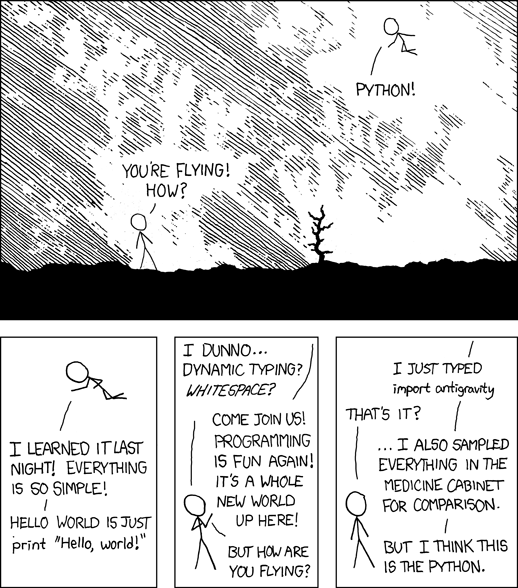
\includegraphics[height=8.5cm]{fig/xkcd.png}
\end{frame}

\begin{frame}\frametitle{Presentando Python}
	\begin{itemize}
		\item Dos versiones: 2.7 y \textbf{3.6}
		\item Libre, abierto y gratuito, con una comunidad enorme $\rightarrow$ todo a golpe de Google.
		\item Mil y una librerías abiertas y gratuitas.
		\item Rápido y fácil de escribir, puede ser lento de ejecutar.
	\end{itemize}

	Para escribirlo: Spyder, cuadernos Jupyter, Pycharm, VS Code, Atom, Geany, Notepad++...
\end{frame}

\subsection{Librerías importantes}

\begin{frame}\frametitle{Librerías importantes}
	\begin{figure}
		\subfigure{
\includegraphics[height=1cm]{fig/numpy.png}}
		\subfigure{
\includegraphics[height=1cm]{fig/scipy.png}}
		\subfigure{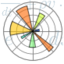
\includegraphics[height=1cm]{fig/matplotlib.png}}
		\subfigure{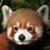
\includegraphics[height=1cm]{fig/pandas.jpg}}
		\subfigure{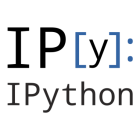
\includegraphics[height=1cm]{fig/ipython.png}}
	\end{figure}

	\centering
	\textbf{Numpy}: cálculo numérico

	\textbf{Scipy}: cálculo científico

	\textbf{Matplotlib}: graficado
	
	\textbf{Pandas}: análisis de datos
	
	\textbf{IPython}: consola interactiva
\end{frame}

\subsection{Programación orientada a objetos}

\begin{frame}\frametitle{Programación orientada a objetos}
	Un \textbf{objeto} tiene \textbf{métodos} (``funciones'') y \textbf{atributos} (``variables'') que lo constituyen.

	\begin{itemize}
		\item \texttt{A.shape}
		\item \texttt{z.conjugate()}
		\item \texttt{v.reshape((3,4))}
	\end{itemize}

	Todo Python trabaja con objetos\footnote{\tiny (hasta donde yo sé)}
\end{frame}


\section{Sintaxis básica de Python}

\begin{frame}\frametitle{Tipos}
	\centering
	\begin{tabular}{ccc}
		Entero 				& \texttt{integer} 			& \texttt{1} \\
		Con coma flotante	& \texttt{float} 			& \texttt{1.} \\
		Complejo 			& \texttt{complex} 			& \texttt{1. + 2j} \\
		Booleano 			& \texttt{boolean} 			& \texttt{True} \\
	\end{tabular}
\end{frame}

\begin{frame}\frametitle{Contenedores}
	\textbf{Cadenas} $\rightarrow$ \texttt{s = "perro"}

	\textbf{Listas} $\rightarrow$ \texttt{l = [1, 'perro', True]}

	\textbf{Tuplas} $\rightarrow$ \texttt{t = (1, 'perro', True)}

	\textbf{Diccionarios} $\rightarrow$ \texttt{d = \{ '1': 2, 'el': 'perro'\}}

	Ojo: los índices van de \texttt{0} a \texttt{n-1}, como en C: 
	\begin{itemize}
		\item \texttt{s[0] = 'p'}
		\item \texttt{l[-1] = True}
		\item \texttt{t[3]} no existe
		\item \texttt{d['el'] = 'dog'}
	\end{itemize}
\end{frame}

\subsection{Sentencias de control}

\begin{frame}{Sentencias de control}

\begin{exampleblock}{Condición: \texttt{if-elif-else}}
	\lstinputlisting[language=Python]{code/if.py}
\end{exampleblock}

\end{frame}

\begin{frame}{Sentencias de control}

	\begin{exampleblock}{Bucle: \texttt{for}}
		\lstinputlisting[language=Python]{code/for.py}
	\end{exampleblock}
	
\end{frame}

\begin{frame}{Sentencias de control}

	\begin{exampleblock}{\textsl{List comprehensions}}
		\lstinputlisting[language=Python]{code/list_comprehension.py}
	\end{exampleblock}
	
\end{frame}

\section{Numpy: el \texttt{ndarray}}

\section{Scipy}

\section{Matplotlib.pyplot}

\end{document}
